% Mirror: https://github.com/SIGma-UIUC/presentation-format
% --------------------------------------------------------------------
% This is a simple Beamer document that uses beamerthemesigma.sty
% Reading the comments should help you create a presentation even if
% you've never used Beamer before.
% --------------------------------------------------------------------

% Set our document class to Beamer
\documentclass[aspectratio=169]{beamer}

% Some packages for nice font encodings in the final PDF
\usepackage[utf8]{inputenc}
\usepackage[T1]{fontenc}

% From Jeff E
\usepackage{algo}

% Some more macros
\usepackage{sigmastyle}

% Citations
\usepackage{cite}

% To insert images
\usepackage{graphicx}

% Useful packages from the AMS
\usepackage{amsmath,amssymb,amsthm}

\usepackage[normalem]{ulem}

% Package for code highlighting
\usepackage{minted}
\setminted{linenos=true, breaklines=true, breakanywhere=true, style=default}
\usemintedstyle{monokai}

% Set a title
\title{Computational Combinatorics and Canonical Deletions}

% Set a subtitle if you desire
\subtitle{\cite[Stolee]{CanonicalDeletions} and \cite[Stolee]{SmallGraphs}}

% Whoever worked on the presentation:
\author{Hassam}

% A date, if you'd like.
\date{}

% An institute name, if you're so inclined
% \institute{University of Illinois Urbana-Champaign}

% Use the SIGma theme for this Beamer presentation
\usetheme{sigma}
% --------------------------------------------------------------------

% Begin document
\begin{document}

% Beamer calls each slide a "frame", defined within the environment:
% \begin{frame}
%   <frame content here>
% \end{frame}

% This frame is just the title.
\begin{frame}
\titlepage
\end{frame}

% A frame with the table of contents.
% This frame's title is "Outline".
\begin{frame}{Outline}
  \tableofcontents
\end{frame}

\section{Motivation}
\frame{\sectionpage}
\begin{frame}{Generating Objects}
    \begin{itemize}
        \item We want to count \textcolor{sigma@mainblue}{\emph{things}} \pause
        \item We don't want to miss any \pause
        \item We don't want to count more than we need to
    \end{itemize}
\end{frame}

\begin{frame}{Generalizing Combinatoric Search}
\begin{itemize}
    \item Start at a base object \pause
    \item Augment the object \pause
    \item Watch out for symmetries (\textcolor{sigma@mainblue}{\emph{isomorphisms}})
\end{itemize}
\end{frame}

\begin{frame}{Finding all Permutations}
    Let's find all permutations of the list [1, 2, 3] 
\begin{itemize}
    \item What's our base object? \pause
    \item Empty list: [] \pause
    \item What do we add next?
    \begin{itemize}
        \item Items: 1, 2, 3
    \end{itemize}
    \item Generate: 
    \begin{itemize}
        \item $[1], [2], [3]$ \pause
        \item $[1, 2], [1, 3], [2, 1], [2, 3], [3, 1], [3, 2]$ \pause
        \item $[1, 2, 3], [1, 3, 2], [2, 1, 3], [2, 3, 1], [3, 1, 2], [3, 2, 1]$ \pause
    \end{itemize}
\end{itemize}
    \vspace{20pt}
    \textcolor{sigma@alertred}{What breaks if we do this with subsets?}
\end{frame}

\section{Augmentations and Deletions}
\frame{\sectionpage}

\begin{frame}{}
    \begin{figure}
        \centering
        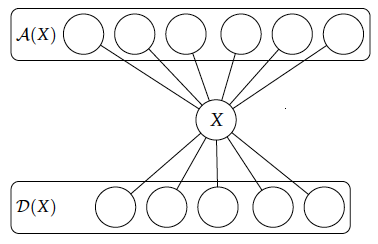
\includegraphics[width = 0.8\textwidth]{aug_delete.png}
    \end{figure}
\end{frame}

\begin{frame}{}
    \begin{figure}
        \centering
        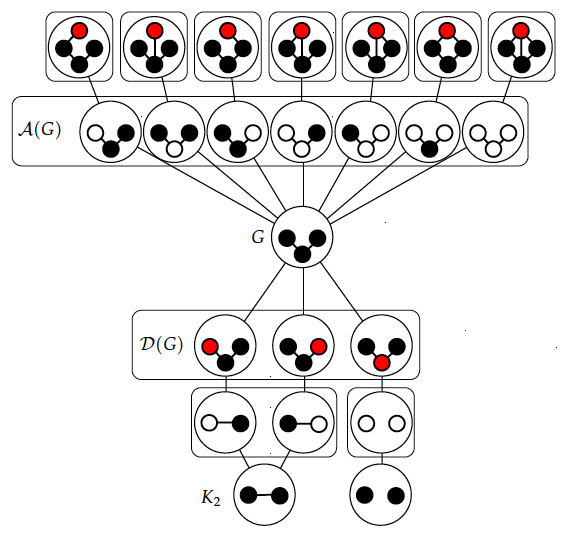
\includegraphics[width = 0.7\linewidth]{aug_delete_k2.png}
    \end{figure}
\end{frame}

\begin{frame}{Removing symmetries (isomorphisms)}
    What if we filtered out local isomorphisms? Is that sufficient? \pause
    \begin{figure}
        \centering
        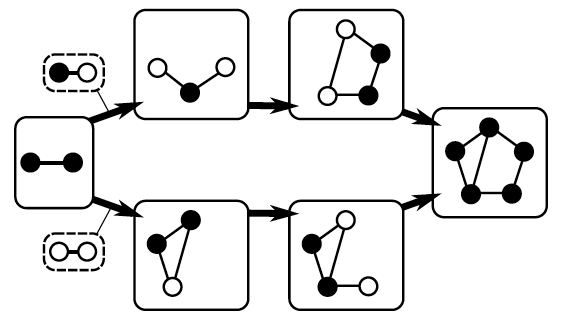
\includegraphics[width = 0.7\linewidth]{isomorph.png}
    \end{figure}
\end{frame}

\section{Canonical Deletions}
\frame{\sectionpage}

\begin{frame}{The Problem}
    We have a way to label every graph and check if they are isomorphic, but this is slow, especially as our search space expands. Going up our list of augmentations, our search space explodes. \pause 

    \hfill
    
    What if we worked down our search space?
\end{frame}

\begin{frame}{Canonical Labels}
    In the process of checking whether two graphs are isomorphic, we generate a canonical label. We can define a canonical labelling as a function such that if $g \cong g'$ then $c(g) = c(g')$, and each element in the co-domain has a ``name''. \pause

    \hfill

    What's an obvious canonical labelling for subsets? 
\end{frame}

\begin{frame}{Canonical Deletions}
    The key idea: Every single canonical labeling has a specific set of deletions and augmentations associated with it. What if we chose one of the deletions to be the correct one? 
\end{frame}

\begin{frame}{A Subset Example}
\begin{itemize}
    \item Let's define the canonical labelling for a set to be the elements of the set in lexicographic order. \pause 
    \item Let's define the canonical deletion for a set to be removing it's smallest lexicographic element. \pause
    \item \textcolor{sigma@alertred}{What's the canonical deletion of $\{3, 4, 1, 2\}$?} \pause
    \item \textcolor{sigma@mainblue}{\{2, 3, 4\}}
\end{itemize}
\end{frame}

\begin{frame}{}
    \begin{figure}
        \centering
        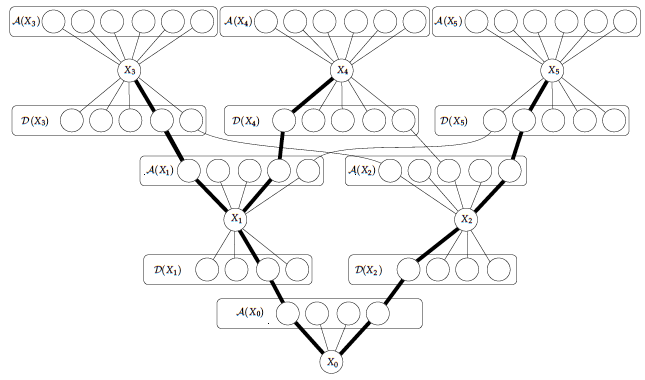
\includegraphics[width = \linewidth]{canonical_deletions.png}
    \end{figure}
\end{frame}

\begin{frame}{Canonical Deletion Algorithm}
    \begin{nalgo}
    \underline{\textsc{CanonicalDeletion}($n, X$)}:
    \\\label{}  \textbf{if} Bad($X$): \hspace{20.5pt}\Comment{Short Circuit Optimization} \+
    \\\label{}      \textbf{return} \-
    \\\label{}  \textbf{if} Solution($X$): \+
    \\\label{}      \textbf{output} $X$ \-
    \\\label{}  \textbf{for all} augmentations $A \in {\mathcal A}(X)$, up to isomorphism: \+
    \\\label{}      $D \leftarrow \delta(A)$ \hspace{15.5pt}\Comment{Get the corresponding deletion}
    \\\label{}      $Y \leftarrow {\mathcal D}^{-1}(D)$ \Comment{Find the object that corresponds to that deletion}
    \\\label{}      $D' \leftarrow {\mathrm{del}}(Y)$ \hspace{3pt}\Comment{Compute its canonical deletion}
    \\\label{}      \textbf{if} $D \cong D'$: \hspace{11.5pt}\Comment{Check that they match} \+
    \\\label{}          \textbf{call} CanonicalDeletion($n, Y$) \-\-
    \\\label{} \textbf{return}
    \end{nalgo}
\end{frame}

\begin{frame}{A Specific Example}
    \begin{itemize}
        \item Let us consider a specific example: \textcolor{sigma@mainblue}{\emph{Generating Graphs}} with $n$ nodes\pause
        \item Restrictions:
        \begin{itemize}
            \item $\Delta(G) \leq 4$: Nodes have maximum degree 4
            \item $\chi(G) \leq 3$: Nodes have chromatic color of at most 3
        \end{itemize}
    \end{itemize}
\end{frame}

\begin{frame}{A Specific Example}
    \begin{nalgo}
    \underline{\textsc{GraphCanonicalDeletion}($n, G$)}:
    \\\label{}  \textbf{if} $\Delta(G) \geq 5$ \textbf{or} $\chi(G) \geq 4$ \textbf{or} $n(G) > n$: \+
    \\\label{}      \textbf{return} \-
    \\\label{}  \textbf{if} $n(G) \equiv n$ \textbf{and} $\Delta(G) \leq 4$ \textbf{and} $\chi(G) \leq 3$: \+
    \\\label{}      \textbf{Output} $G$ \-
    \\\label{}  \textbf{for all} $S \subseteq V(G)$: \+
    \\\label{}      $H \leftarrow G + v_S$ \hspace{20.5pt}\Comment{Augment the graph}
    \\\label{}      $(H, v') \leftarrow {\mathrm{del}}(H)$ \Comment{Compute its canonical deletion}
    \\\label{}      \textbf{if} $v_S$ and $v'$ are the same vertex: \+
    \\\label{}          \textbf{call} CanonicalDeletion($n, H$) \-\-
    \\\label{} \textbf{return}
    \end{nalgo}
\end{frame}

\begin{frame}{So what?}
    What guarantees do we have? \pause
    \begin{enumerate}
        \item Every object that has the desired property we are looking for is visited only once \pause
        \item We can use pruning to avoid visiting any objects that don't have this property more than once \pause
        \item Most importantly, this process is entirely local. We can parallelize it. 
    \end{enumerate}
\end{frame}

\section{The Reconstruction Conjecture}
\frame{\sectionpage}

\begin{frame}{An \sout{Open}(?) Problem in Graph Theory}
    The reconstruction conjecture was posed by Kelly and Ulam as something to play with while Ulam was working on the atomic bomb. There are some papers claiming to have proven this conjecture true, but they go above my head and I can't find any reputable source verifying them. 
\end{frame}

\begin{frame}{Graph Decks}
    Given a graph $G$, its deck is the multi-set of graphs $H$ such that $H$ is isomorphic to a single vertex deleted subgraph of $G$.
    \begin{figure}
        \centering
        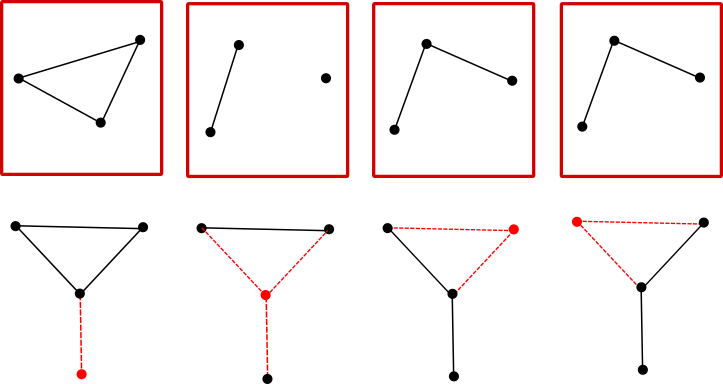
\includegraphics[width = 0.9\linewidth]{deck.png}
    \end{figure}
\end{frame}

\begin{frame}{Are decks all you need?}
    In other words: if $G$ and $G'$ have isomorphic decks, are $G$ and $G'$ isomorphic? 
\end{frame}

\begin{frame}{Naive Testing}
    We could generate every graph of order $n$ and do pairwise comparisons of their decks. This is not a lot of programming, sage, geng, etc. Generating graphs is not too bad, we will probably have to do this anyway. This is a lot of comparisons though. 
\end{frame}

\begin{frame}{Testing smarter}
Suppose we had two distinct graphs with the same deck, then those two graphs must come from the same set of augmentations/deletions. To check that a $n$ vertex graph is reconstructible, we only need to compare it to the augmentations that come from its canonical deletion! 

\hfill

In practice, we go from $n^2$ comparisons to approximately $n \log n$ comparisons.  
\end{frame}

\begin{frame}{Results}
    McKay, when he first created the Nauty library, was able to show that the theorem holds for all graphs of up to order 11. This was in 1997. Can we do better using modern hardware? I think we can. \cite{McKay1997SmallGA} \pause

    \hfill

    Update: in 2021, McKay repeated this inquiry, with a few additions, using modern computers. He was able to show the reconstruction theorem holds for all graphs up to order 13. It took him 1.5 years of compute-time though. \cite{McKaySmallGraphsReconstruction}
\end{frame}



% Remove this slide if you came up with all the material yourself
\begin{frame}{Bibliography}
    \bibliographystyle{alpha}
    {\scriptsize \bibliography{refs}}
\end{frame}

\end{document}